%	CHAP Docker%----------------------------------------------------------------------------------------

\chapterimage{blue-chapter-head_4-reduced.pdf} % Chapter heading image

\chapter{Instant refresh}\label{chap:InstantRefresh}
Instant Refresh (IR) was introduced in MetaR 2.0.\index{New in MetaR 2.0} This feature allows users to make changes in their scripts and see results updated seamlessly. Instant refresh supports both MetaR Analysis and composable R scripts.  
Changes in Analysis or RScripts are automatically detected and copied to a new Analysis node called \texttt{Instant refresh}. Based on configurable settings, either a normal run configuration with a local R installation, or a new docker container is started to execute the instant refresh code. Executing the code regenerates tables or plots and updates the display. Users can follow progress of the refresh in the Instant Refresh tool. This Chapter describes this feature in more details. Instant Refresh was developed by Alexander Pann during a summer internship in the lab.

\section{Usage}
IR is activated by default but this behavior can be opted out in the preferences.
To allow re-executing code in RScript nodes make sure that you are using
the install or load expression (type \texttt{installOrLoad} and use auto-complete) for loading R libraries in the script (see Section~\ref{sec:installOrLoad}). This expression is needed for locating all the libraries
that need to be loaded when the code is re-executed. It should be used as a
replacement for the R commands \texttt{install.packages}, \texttt{library} or \texttt{require}.

\begin{remark}
Note that not all expressions are considered changes when calculating the list of changes to be re-executed. Some nodes are ignored including empty lines, comments and \texttt{Save Session} expressions.
\end{remark}

\begin{figure}[h!tbp]
  \centering
  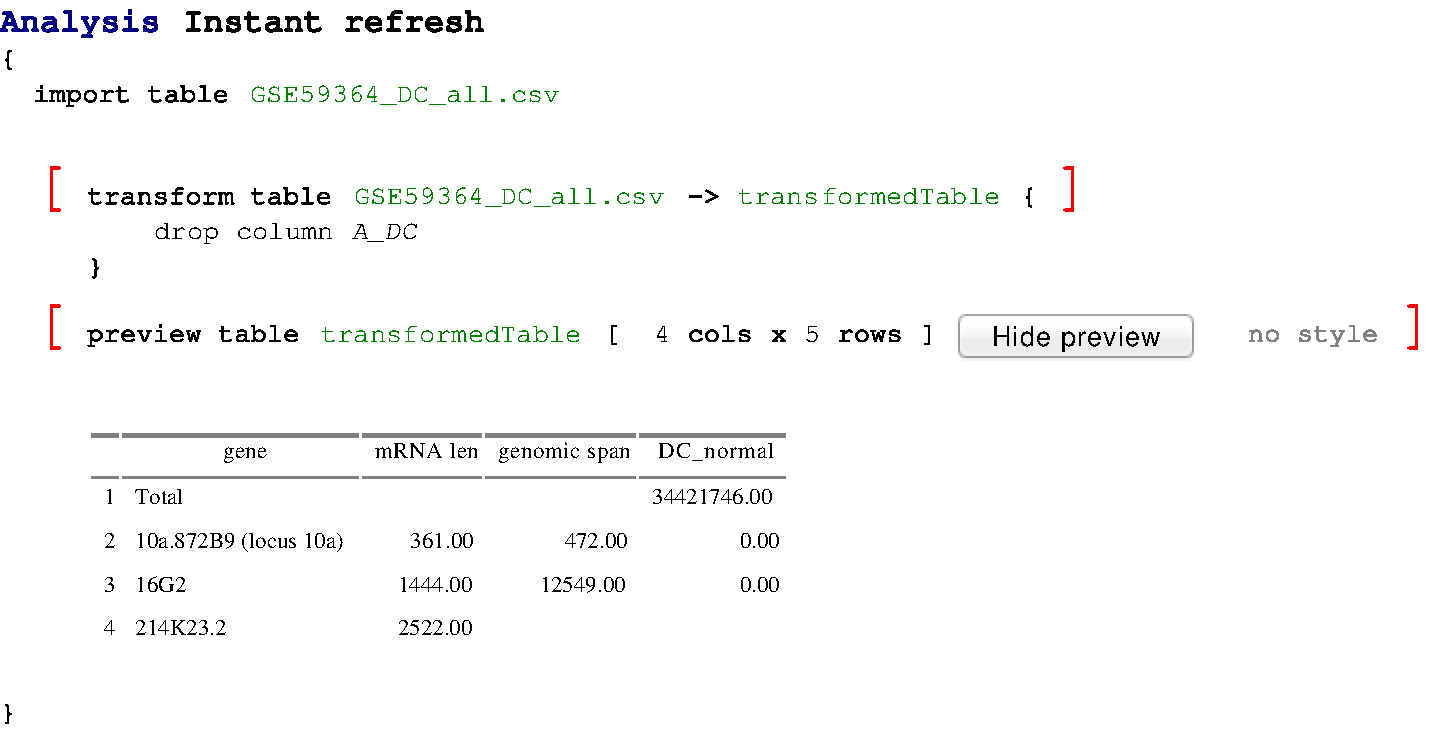
\includegraphics[width=\figWidthWide]{figures/IRChangedStatements.pdf}
\caption[Visualize Changes]{\textbf{Visualize Changes} Assume a change is made in the transform table statement (drop column). The figure shows the statements that need to be re-executed are surrounded by red brackets. You can visualize changes by by placing the cursor over the point of change and using the 'Show Statements That Would Be Affected by a Change'' intention.}
\end{figure}

\subsection{Instant refresh node}
The Analysis node \texttt{Instant refresh} is a node that is automatically inserted in the current model and is populated with all expressions/statements
that have to be re-executed. 

\begin{remark}
Note that changes made manually in the Instant Refresh node are ignored and will be deleted and replaced the next time IR is triggered.
\end{remark}


\section{IR Preferences}
The preferences can be found in the Preferences/Settings MPS menu (\menu{MPS > Preferences > Other Settings > InstantRefresh} on Mac, \menu{MPS > Settings}\allowbreak
\menu{Other Settings} \menu{InstantRefresh} on PC). 

There are a few options that can be changed:

\begin{figure}[h!tbp]
  \centering
  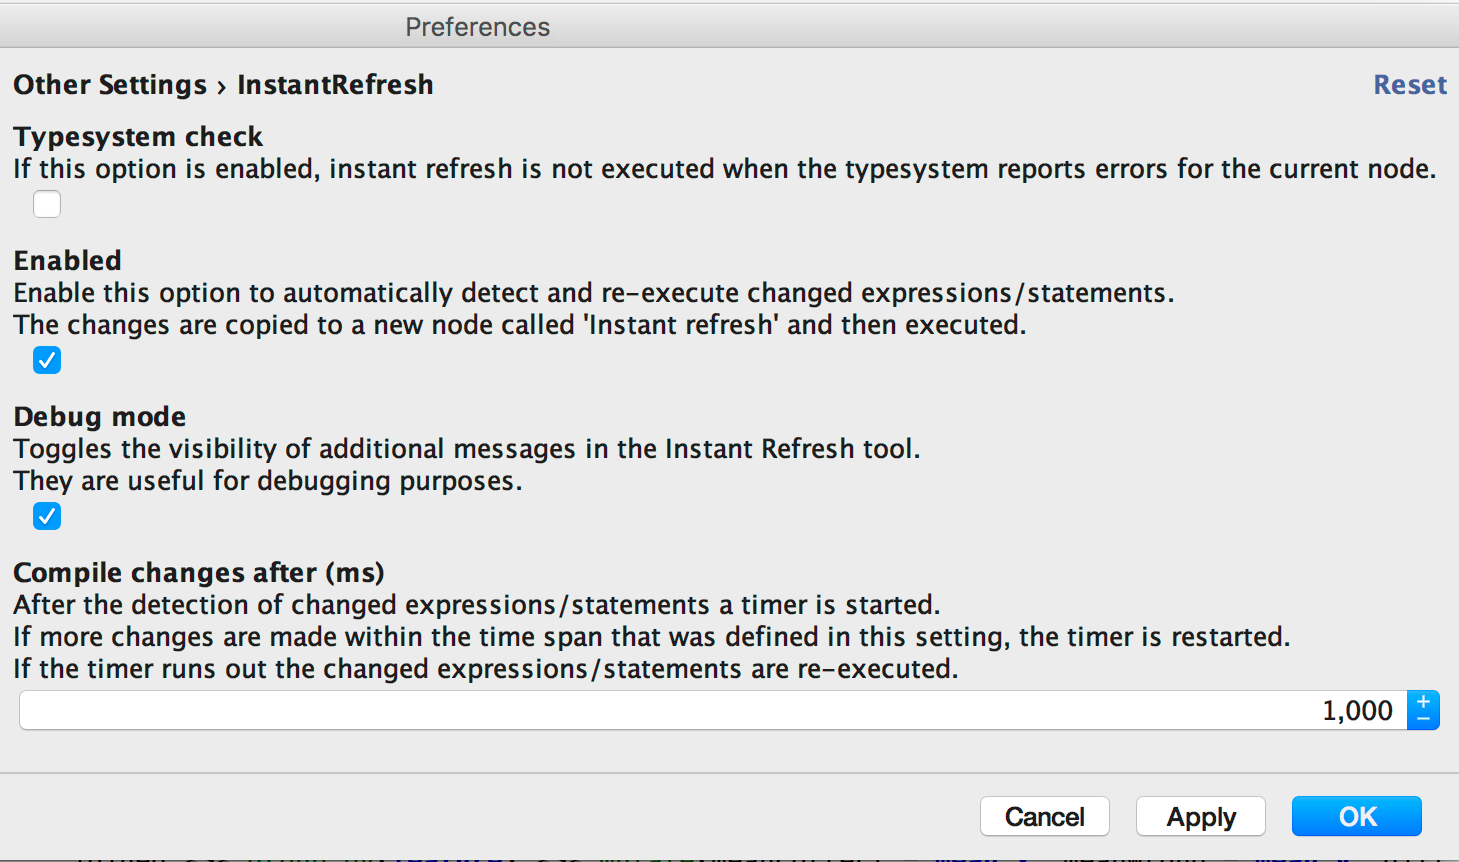
\includegraphics[width=\figWidthWide]{figures/IRPreferences-2.png}
\caption[Instant Refresh Settings]{\textbf{Instant Refresh Settings} This dialog is available under MPS Preferences/Settings and controls the behavior of IR.}
\end{figure}

\begin{enumerate}
	\item \textbf{Type system check}. 
	If this option is enabled, instant refresh is not executed when the type system 	reports errors for the current node.
	\item \textbf{Enabled}. Toggle this option to activate or deactivate IR.
	\item \textbf{Debug mode}.
	Toggles the visibility of additional messages in the IR tool. These messages 			are helpful for debugging purposes.
	They also give some additional information, for instance explaining in some cases why IR was not 	 executed (e.g. the feature is not enabled, a pause expression is active..).
	Additionally it outputs the standard output of the currently executing script 	that would normally be found in the Run tab console.
\end{enumerate}

\section{Tool}
The IR tool is a tab that is located at the bottom left of the screen. It displays a message when R code is generated and executed as
well as the execution time of both of these phases. If the debugging mode is activated, the output is way more verbose.

\section{pause instant refresh}
Although IR can be disabled in Preferences, there is sometimes a need to pause it only for the current script. For instance, this is useful if you know that you need to add several new statements to a script and do not want MetaR to attempt executing incomplete scripts. RScript nodes have
a built-in expression to achieve this. It can be activated by typing \texttt{pause instant refresh} and using auto-complete anywhere in the script. When the \texttt{pause instant refresh} expression is present in a script, IR will not attempt to execute this script. You can resume instant refresh by deleting the expression.

\begin{remark}
The \texttt{pause instant refresh} expression can only be used once per script because it affects the whole script.
\end{remark}

\section{Sessions}
To accelerate the re-execution of R code, sessions are used. Sessions are files with the extension ".RDa" and are saved in a sub folder of the results directory.

They contain an external representation of R objects that can be used for restoring the R environment. Every statement in an Analysis node automatically saves a new session file after the execution of the statement. In RScript nodes save session expressions can be inserted manually. They can only be inserted at the root level of the script and not inside nested expressions (e.g. if statements, functions, blocks...). When a change is made, the nearest saved session is loaded and changed expressions are only executed if they are located after this expression. All sessions in the current model can be removed by using the use the "Invalidate Sessions" intention (\intentionLightBulb)  and new session files will be created on the next run of IR.
 
\begin{SCfigure}
  \centering
  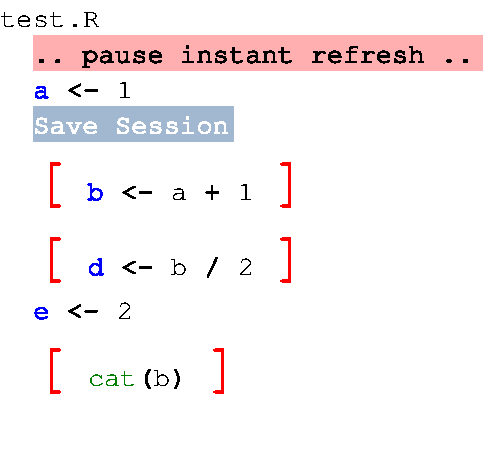
\includegraphics[width=\figWidthSmall]{figures/IRPauseAndSessionExpression.pdf}
\caption[Sessions Affect the List of Changed Nodes]{\textbf{Sessions Affect the List of Changed Nodes.} A change was made in the expression after the \texttt{Save Session} expression and therefore the statement above does not have to be re-executed.}
\end{SCfigure}
